\section{Round Robin 2}

Para la implementacion de $Round Robin 2$ se utilizo como base la implementacion original de $Round Robin$, a partir de esta se modifico segun los nuevos requerimientos.

\subsection{Codigo}

\subsubsection{Class Declaration}
\begin{lstlisting}[language=C++, breaklines=true]
class SchedRR2 : public SchedBase {
	public:
		SchedRR2(std::vector<int> argn);
        ~SchedRR2();
		virtual void load(int pid);
		virtual void unblock(int pid);
		virtual int tick(int cpu, const enum Motivo m);
	private:
		int* quantum;
		int* cycles;
		std::vector<std::queue<int> > q;
		std::vector<int> totalLoad; // buscar otra estructura?
		std::map<int,int> CPUBlockedTask;

		int getCPU();
};
\end{lstlisting}

A diferencia de $Round Robin$, en este caso tenemos una cola de tareas por CPU, la carga total por procesador y un $map$ que sirve para tomar nota de los procesos bloqueados y del procesador que tiene asingado.

\subsubsection{Constructor y Destructor}
\begin{lstlisting}[language=C++, breaklines=true]
SchedRR2::SchedRR2(vector<int> argn) {
	// Round robin recibe la cantidad de cores y sus cpu_quantum por parametro
	quantum = new int[argn.size()-1];

	for (int i = 0; i < argn[0]; ++i) {
		q.push_back(queue<int>());
		totalLoad.push_back(0);
	}

	for (int i = 1; i < (int) argn.size(); i++) {
		quantum[i-1] = argn[i];
	}

	cycles = new int[argn[0]];
}

SchedRR2::~SchedRR2() {
	delete[] cycles;
	delete[] quantum;
}
\end{lstlisting}

Aqui inicalizamos las estructuras de datos utlizando los parametros recibidos, inicialmente la carga es cero para todos los procesadores.

\subsubsection{Load y Unblock}
\begin{lstlisting}[language=C++, breaklines=true]
void SchedRR2::load(int pid) {
	int cpu = getCPU();
	q.at(cpu).push(pid);
	totalLoad[cpu]++;
}

void SchedRR2::unblock(int pid) {
	q.at(CPUBlockedTask[pid]).push(pid);
}

int SchedRR2::getCPU() {
	int cpu = 0;
	int i = 1;
	for (vector<int>::iterator it = ++totalLoad.begin() ; it != totalLoad.end(); ++it) {
		if (*it < totalLoad.at(cpu)) {
			cpu = i;
		}
		i++;
	}
	return cpu;
}
\end{lstlisting}

En el caso del $load$ tenemos que buscar la CPU que tenga menor carga total, para hacer esto contamos con la funcion auxiliar \texttt{getCPU()} la cual se encarga de recorrer el vector \texttt{totalLoad} en busca del procesador adecuado. Una vez obtenida dicha CPU, procedemos a agregar la tarea a su cola y aumentamos la carga total en uno.

En el caso del $unblock$ hacemos uso del $map$, simplemente volvemos a agregar la tarea a la CPU donde se produjo la llamada bloqueante, ya que la tarea necesita haber estado bloqueada para llamar a $unblock$ el $map$ siempre va a dar una CPU valida.

\subsubsection{Tick}
\begin{lstlisting}[language=C++, breaklines=true]
int SchedRR2::tick(int cpu, const enum Motivo m) {
	if (m == EXIT || m == BLOCK) {
		// Si la tarea termino, se la quita de la carga total.
		// Si se bloqueo, se toma nota de la CPU actual para poder
		// agregarla nuevamente cuando se desbloquee.
		if (m == EXIT) {
			totalLoad[cpu]--;
		} else {
			CPUBlockedTask[current_pid(cpu)] = cpu;
		}

		// Si el pid actual termino, sigue el proximo.
		if (q.at(cpu).empty()) return IDLE_TASK;
		else {
			int sig = q.at(cpu).front(); q.at(cpu).pop();
			cycles[cpu] = quantum[cpu];
			return sig;
		}
	} else {
		if (current_pid(cpu) == IDLE_TASK && !q.at(cpu).empty()) {
			int sig = q.at(cpu).front(); q.at(cpu).pop();
			cycles[cpu] = quantum[cpu];
			return sig;
		} else {
			cycles[cpu]--;

			if (cycles[cpu] == 0) {
				if (q.at(cpu).empty()) {
					cycles[cpu] = quantum[cpu];
					return current_pid(cpu);
				} else {
					int sig = q.at(cpu).front(); q.at(cpu).pop();
					q.at(cpu).push(current_pid(cpu)); // re-add to queue
					cycles[cpu] = quantum[cpu];
					return sig;
				}
			} else {
				return current_pid(cpu);
			}
		}
	}
}
\end{lstlisting}

El $tick$ opera de manera casi identica a la del de $Round Robin$, la unica diferencia es la cola de tareas individual por CPU, como manipular los bloqueos y el fin de las tareas.

Si el $tick$ es normal (es decir, no es un bloqueo ni un fin de ejecucion), se procede igual que $Round Robin$, con la diferencia que en vez de usar la cola global \texttt{q} usamos la cola correspondiente a la CPU actual. Si por el contrario recibimos un \texttt{BLOCK} guardamos la CPU del proceso actual en el $map$, en el caso de \texttt{EXIT} procedemos a reducir la carga del CPU actual en uno, en ambos casos luego procedemos a desalojar la tarea, cargar la siguiente (si es que la hay) y resetear el quantum.

\subsection{Lote de tareas de prueba}

Para ver el beneficio de la migracion de proceso, vamos a probar con las siguientes tareas:

\begin{itemize}
	\item Tarea 0: 100 ciclos de CPU, 0 llamadas bloqueantes
	\item Tarea 1: 50 ciclos de CPU, 0 llamadas bloqueantes
	\item Tarea 2: 100 ciclos de CPU, 0 llamada bloqueante
	\item Tarea 3: 50 ciclos de CPU, 0 llamadas bloqueantes
	\item Tarea 4: 100 ciclos de CPU, 0 llamadas bloqueantes
\end{itemize}

\begin{figure}[h]
    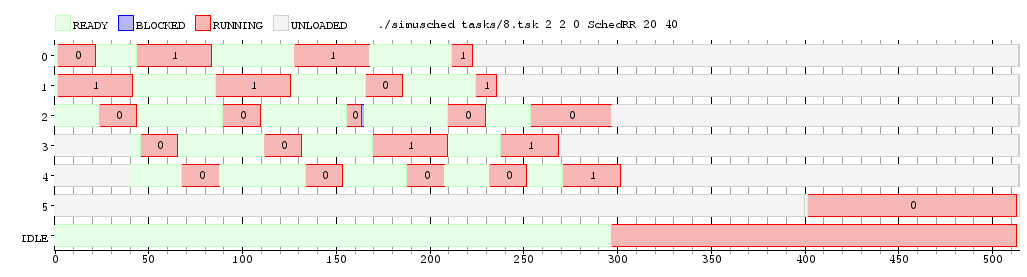
\includegraphics[width=\linewidth]{images/8_quantumRR.png}
    \label{fig:Task Consola}
    \caption{Round Robin}
\end{figure}

\begin{figure}[h]
    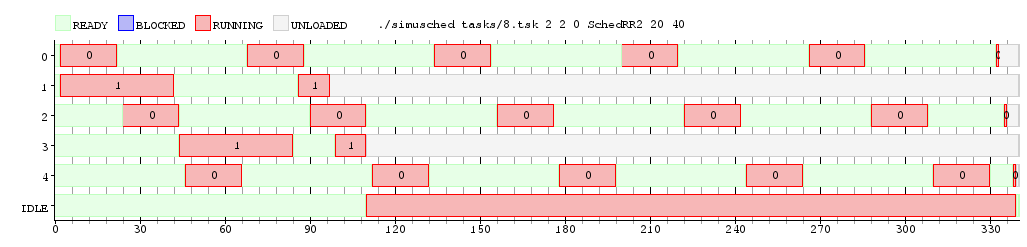
\includegraphics[width=\linewidth]{images/8_quantumRR2.png}
    \label{fig:Task Consola}
    \caption{Round Robin 2}
\end{figure}

\pagebreak

En este caso podemos ver claramente que la migracion de procesos entre nucleos ayuda a reducir ampliamente el tiempo total en el sistema de varias tareas. Debido a nuestra implementacion, los procesos que toman 100 ciclos van a parar a la primer CPU, mientras que los que toman 50 ciclos son asignados a la segunda CPU. Con respecto a temas de $latencia$, podemos ver que $Round Robin 2$ tiene mejor comportamiento que $Round Robin$, sin embargo, esta distribucion de tarea impacata negativamente a la concurrencia ya que una vez concluidas las tareas 1 y 3, la segunda CPU entra en estado oscioso y el scheduler no le asigna mas procesos. Esto ultimo hace que la ultima tarea concluya aproximadamente a los 230 ciclos en el caso de $Round Robin$, mientras que en $Round Robin 2$ la ultima tarea concluye aproximadamente a los 340 ciclos.

Para ver un caso donde la migracion de procesos no mejora significativamente los tiempos totales de ejecucion, tenemos el siguiente caso:

\begin{itemize}
	\item Tarea 0: 100 ciclos de CPU, 0 llamadas bloqueantes
	\item Tarea 1: 50 ciclos de CPU, 50 llamadas bloqueantes
	\item Tarea 2: 100 ciclos de CPU, 0 llamada bloqueante
	\item Tarea 3: 50 ciclos de CPU, 50 llamadas bloqueantes
	\item Tarea 4: 100 ciclos de CPU, 0 llamadas bloqueantes
\end{itemize}

\begin{figure}[h]
    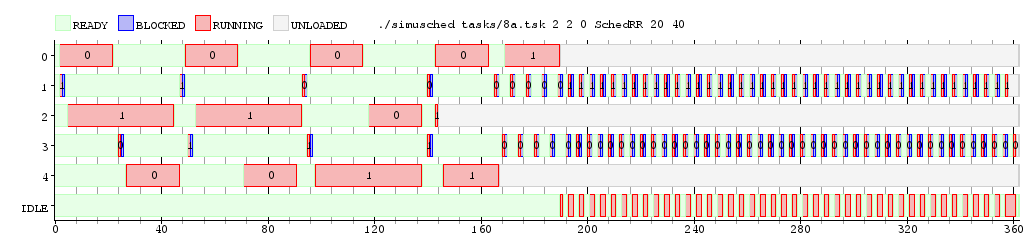
\includegraphics[width=\linewidth]{images/8a_quantumRR.png}
    \label{fig:Task Consola}
    \caption{Round Robin}
\end{figure}

\pagebreak

\begin{figure}[h]
    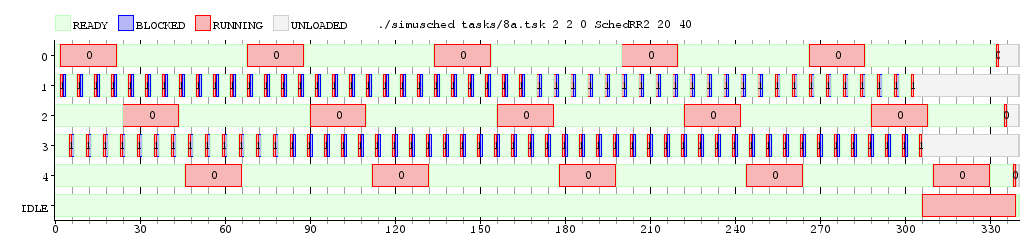
\includegraphics[width=\linewidth]{images/8a_quantumRR2.png}
    \label{fig:Task Consola}
    \caption{Round Robin 2}
\end{figure}

Aqui podemos apreciar que la migracion de procesos entre nucleos no nos aporta una mejora significativa, la cantidad de llamadas bloqueantes es suficientemente grande como para nulificar cualquier tipo de beneficio de la migracion entre procesos. Incluso podemos apreciar que la migracion hace que si bien algunas tareas concluyan en menor tiempo, durante una gran cantidad de tiempo tenemos algun nucleo en estado oscioso en el caso de $Round Robin$.
